%!TEX TS-program = xelatex
%!TEX encoding = UTF-8 Unicode

\documentclass{../Dissertate}

\begin{document}

\doublespacing

\setcounter{chapter}{2} % This chapter minus 1
\chapter{Perceptual Similarity vs. Conceptual Knowledge in Induction}

\section{Introduction}

In Chapter 1, I discussed how people can
draw on different sources of information in induction.
In this chapter, I report a pair of experiments in which
two such sources --- perceptual similarity,
and conceptual knowledge in the form of category membership ---
are placed into conflict.
This was done using a mouse tracking version of
\citegap{Gelman1986}{'s} inductive triad task.
In Experiment 1, participants learned a biological property of
different species in the natural world, and were asked to
project each property to one of two species,
one of which belonged to the same taxonomic group as the base species.
In the conflict condition, but not the control condition,
the base and the foil species looked alike,
and so perceptual cues conflicted with conceptual knowledge.
In Experiment 2, participants completed a similar task,
but using artificial categories, learned at the start of the experiment.
I also manipulated the nature of the properties
participants reasoned about in Experiment 2, between participants,
to reveal how this modulated participants' inferences.

As discussed in Chapter 1,
theories of inductive reasoning can be organised into two groups.
One class of theory relies on conceptual knowledge
about the categories to which different entities belong,
and the relations between these categories.
Category membership is perhaps the most fundamental 
such form of conceptual knowledge that we can use as the basis for induction.
According to contemporary accounts of categorisation
\citep[see][]{Murphy2004,Rosch1988},
a category consists of a set of entities that have attributes in common.
Therefore, if we know the category to which something belongs,
we may believe that it has attributes
that we know are found in other members of that category
\citep{Murphy2004,Osherson1990}.
That adults can reason in this way has never been in question,
and indeed this idea is central to the very notion of categorisation
\citep{Mill1856,Gelman1986}.
This principle applies equally to inferences about people,
where it is better known as \emph{stereotyping}
\citep{Greenwald1995,Oakes1994}.
% The evidence that we do use knowledge about categories when reasoning
% is considerable, and indeed this should be self-evident,
% and so will not be reviewed in detail here.
% Few results in literature on inductive reasoning in adults
% \citep[see][for reviews]{Feeney2007,Hayes2010}, for example,
% can be accounted for without recourse to category-based inference.
Strikingly, people rely on categorical information
even when it is disadvantageous to do so.
Murphy and Ross \citep{Murphy2012,Murphy2010,Malt1995,Murphy1994}
showed, for instance, that when it is not certain
to which category an entity belongs,
participants nevertheless reason on the basis
of it belonging to the most likely category.
\citet{Mishra2010} also report a \emph{border bias} phenomena:
distant locations in the same state (for instance New York City, and Buffalo, New York) 
are perceived as physically closer, and more likely to share properties,
than closer locations divided by state lines (New York City and Princeton, New Jersey.

% \aside{I could also talk about language, and developmental trends here,
%   but I don't think I will}
Category membership is also at the core of many more sophisticated theories of induction
\citep[i.e.][]{Osherson1990,Griffiths2009,Kemp2009},
which combine information about category membership
with knowledge about the relationships between various categories.

% Similarity
Other theories of induction are not based on category membership.
Similarity between entities is the most common kind of
non-categorical information proposed to underlie induction:
entities that are similar (i.e. that share many features)
are more likely to also share a new feature
than things that are dissimilar.
This principle forms the basis of many feature-based accounts of induction
\citep{Sloman1993,Rogers2004,Sloutsky2004,Fisher2015},
discussed in Chapter 1.
\citet{Fisher2015} draw a distinction between two kinds of similarity,
based on either overlapping perceptual cues,
or on shared features in our mental representations.
With regard to adults' inferences,
the focus has been on the latter, \emph{representational} similarity.
While it is usually assumed that adults
are not swayed by inappropriate perceptual cues,
overlapping features in our mental representations of entities
form the basis of both \citegap{Sloman1993}{'s} Feature Based Induction model,
and \citegap{Rogers2004}{'s} Semantic Cognition accounts of induction.
\citet{Sloutsky2008,Sloutsky2004} propose
an analogous model to explain children's inferences,
based on perceptual similarity.
%% Interestingly, in contrast to findings \citep[i.e.][]{Murphy2012} that
%% reasoning under uncertainty is based on the most likely categorisation only,
%% inferences made under speeded conditions \citep{Chen2013,Verde2005,Newell2010}
%% are usually made on the basis of shared properties,
%% rather than category membership.

Given the importance of conceptual knowledge such as category membership in induction,
why then might perceptual similarity play a role?
One reason is that similarity is a useful proxy for shared category membership:
categories are collections of things that share properties, 
including visible features,
and things which look alike tend to belong to the same category.
Furthermore, regardless of category membership,
attributes tend to be correlated in the real world:
things that share properties we know of
are more likely to also share novel properties
\cite[see, e.g.,][]{Kemp2012}.
For both of these reasons, under many circumstances 
similarity --- even perceptual similarity ---
and conceptual knowledge will support the same inferences.
However, there do exist problems for which
these two kinds of information disagree,
most notably when reasoning about entities
that look more like members of a different category
than members of the category to which they belong
(that is, visually \emph{atypical} category members).
The archetypal examples of such atypical entities are whales,
which are mammals, but bear closer resemblance to fish
than to other mammals.


% Development
This chapter, like the rest of this thesis, focuses on adults' reasoning.
However, there has been little prior research on the role of
simple perceptual cues in adults' inductive reasoning,
perhaps because it would appear self-evident that
adults rely on conceptual knowledge,
or at least representational similarity.
There has been extensive debate, however,
as to whether young children make use of conceptual knowledge at all,
or if their inferences are simply driven by perceptual similarity.

There are a number of reasons to believe that children may rely on perceptual-cues,
rather than conceptual knowledge, in induction.
Conceptual knowledge must be acquired through instruction and experience,
and so early inferences, by which infants and children make sense of the world,
must be driven by a simpler, associative process like visual similarity
\citep{Westermann2013,French2004}.
In recent years, it has also become apparent that
simple associative mechanisms can produce
inferences that are surprisingly complex and flexible \citep{Sloutsky2008,Hinton2014}.
Indeed, \emph{deep neural networks} ---
neural networks, using simple associative principles but with many layers ---
are at the forefront of modern machine learning and artificial intelligence research
\citep{Mnih2013,Hinton2006}.

Sloutsky \citep[i.e.][see \citealp{Sloutsky2003,Sloutsky2010} for reviews]{
  Sloutsky2008,Sloutsky2007,Sloutsky2004a}
has therefore argued that young children's reasoning
is often based on such perceptual cues,
with reliance on conceptual knowledge arising later in development.
In contrast, Gelman 
\citep[i.e.][see \citealp{Gelman2011a,Gelman2004a} for reviews]{
  Gelman2013c,Rhodes2009,Gelman2007a,Gelman1986}
argues that even toddlers
 % \aside{Or younger?}
rely on conceptual knowledge about the world,
and naive theories \citep{Gopnik2003,Carey2009} 
to make inferences about the world around them.

\citegap{Gelman1986}{'s} triad task,
discussed in Chapter 1,
has been widely used as a testing ground
for these competing accounts.
Recall that in this task,
children were presented with images of two entities
(a flamingo and a bat, for instance),
given their labels (``bird'' and ``bat''),
and told a property of each
(``This bird's legs get cold at night'';
``This bat's legs stay warm at night'').
They were also shown a third species
(a blackbird in this example, labelled ``bird'',
but which more closely resembled the bat)
and asked to indicate which property it would have
(``Do this bird's legs get cold at night, like this bird's,
or stay warm at night, like this bat's?'').
\citet{Gelman1986} report that children as young as four
predominantly resist the perceptual cue,
and reason based on shared category membership --
projecting a property from the flamingo to the blackbird,
in this case.
On the other hand, \citet{Sloutsky2007} present results with artificial categories
that seem to show children ignoring category membership
in favour of perceptual similarity.
\citet{Gelman2013c}, however, demonstrate that
this result only holds under certain circumstances,
specifically, when the nature of the learned categories is obscure
and not obviously relevant to the properties being projected
(i.e. a creature's ratio of buttons to fingers).

% Hybrid theory
In Chapter 1, I introduced \citegap{Bright2014a}{'s} hybrid theory of induction.
This proposes that when reasoning inductively,
we can draw on either simple, associative knowledge --- such as similarity ---
or structured knowledge about the relationships between
entities and the categories they belong to.
The distinction in question in the current chapter,
between perceptual cues and simple conceptual knowledge,
is perhaps a more fundamental one than that made by
\citet{Bright2014a} between associative and structured knowledge.
Nevertheless, their hybrid account could easily
be extended to include it.

A prediction that emerges from this extended version of the hybrid theory
is that even adults' inferences may be influenced by perceptual similarity.
To date, there has been little evidence
suggesting that adults' inferences are driven by perceptual cues.
However, as discussed in Chapter 1,
this may in part be because methods used in previous work
were poorly suited to revealing such conflict,
and so in this chapter I explore this question
using the mouse tracking paradigm.
However, previous studies using this triad task
\citep[i.e.][]{Gelman1986,Sloutsky2007,Gelman2013c}
both with adult and child participants,
have only included trials in which perceptual similarity
and conceptual knowledge have conflicted.
Typically, adults overwhelmingly respond on the basis
of conceptual knowledge on such trials,
while the debate has focused on whether children's responses
are driven by conceptual knowledge \citep{Gelman1986,Gelman2013c}
or perceptual similarity \citep{Sloutsky2007}.
By not including trials in which both cues agree, however,
these experiments do not make it possible to see
if adults' reasoning was influenced by perceptual cues
in addition to conceptual knowledge:
when perceptual cues disagree with conceptual knowledge,
participants may be less likely to give the conceptually-cued response,
or slower to do so, or be otherwise conflicted,
than when the cues agree.

Therefore, in this chapter, I present two experiments, with adult participants,
in which perceptual cues either conflict or agree with conceptual knowledge.
If adult induction is in part driven by perceptual cues,
participants should be less likely to generalise
from a base entity to a conceptually-related one
when the alternative, foil entity is visually similar to the base.
Recording participants' mouse cursor trajectories,
it is also possible to investigate how these kinds of information interact over time.
If participants are driven by \emph{either} perceptual similarity
\emph{or} conceptual knowledge on each trial,
they should move the mouse directly to one or other response.
Alternatively, if participants are initially driven by
quickly-available perceptual cues,
but draw on conceptual knowledge later in the reasoning process,
we may see reversal trajectories, as participants
initially move towards the perceptually-cued option,
and change direction mid-trial.






\section{Experiment 1}

In Experiment 1, participants completed
a mouse tracking version of \citegap{Gelman1986}{'s} triad task,
with natural categories.
In the original version of this task, children had to choose
between generalising a property from a base species
to another conceptually-related species,
or to an unrelated but perceptually similar one.
This experiment is, to my knowledge,
the first to include a control condition,
in which both perceptual and conceptual information cue the same response.
Using this experimental manipulation, it is possible to
explore the role these perceptual cues play in reasoning.
Additionally, by recording participants' mouse cursor movements,
the experiment provides a window into processes during reasoning,
rather than just the final inferences participants make.



\subsection{Method}

\subsubsection{Participants}

Fifty nine undergraduate students took part in exchange for course credit.

\subsubsection{Stimuli \& Procedure}

At  the start of the experiment,
participants were presented with a framing story,
based on those used by \citet{Sloutsky2007} and \citet{Gelman2013c}.
This introduced a boy, Mark, who had moved to a country called Elbee,
where his teacher was teaching him
about the plants and animals found there.
They were instructed that they would be told
some of the facts that Mark's teacher had told him,
and shown pictures of three animals.
They were also instructed that their task was to decide,
given a fact about one species,
which of the two other species
this fact was likely to be true for.
This was illustrated using an example.

Participants then completed ten induction trials, in random order.
Induction stimuli were similar to those used by \citet{Gelman1986},
but were created for the current experiment.
They consisted of ten sets of species of plants and animals.
The full set of stimuli used can be found in Appendix~\ref{appendix:exp1_stimuli}.
Each set was made up of a \emph{base} species,
a \emph{correct response} species belonging to
the same super-ordinate category as the base,
and two \emph{foil} species, belonging to a different category:
one that was intended to be
perceptually similar to the base, and one that was not.
Each species was represented in the experiment
by a colour photograph (see Figure~\ref{fig:exp1-screenshot1},
and Appendix~\ref{appendix:exp1_stimuli}).
For each participant, five stimuli sets were randomly chosen as
conflict trials, and presented with the foil
that was perceptually similar to the base.
The remaining sets were designated control trials
and presented with the foil dissimilar to the base.

On each trial, the base was presented
in the centre of the screen,
with a property of that species shown above the image.
Blank genetic properties were used, of the form
``This one has gene 4ew. What else do you think has gene 4ew?''.
After clicking a button marked ``NEXT'' in the bottom centre of the screen,
images of the two possible response species
appeared in the top left and right corners,
with their positions randomised on each trial
(Figure~\ref{fig:exp1-screenshot1}).
Participants responded by clicking on one or other image,
and the position of the mouse cursor was recorded as they did so.

\begin{figure}[pt]
  \centering
  \includegraphics[width=.8\textwidth]{imgs/natural_conflict.png}
  \caption[Screen shot of conflict trial from Experiment 1.]{
    Screen shot of conflict trial from Experiment 1.
    The base image, a striped fish, belongs to the same category as the
    correct response option, the goldfish shown in the top left,
    but is perceptually similar to the foil option,
    the zebra in the top right.}
  \label{fig:exp1-screenshot1}
\end{figure}

\begin{figure}[pb]
  \centering
  \includegraphics[width=.7\textwidth]{imgs/exp1_posttest.png}
  \caption{Screen shot from the post-test check, Experiment 1.
    \label{fig:exp1-screenshot2}}
\end{figure}


After the reasoning trials, participants completed a post-test check.
This was to ensure that participants possessed the appropriate
structured knowledge about the relationships between
the species used.
Each base species was presented twice,
once alongside its corresponding correct response,
which belonged to the same biological category,
and once alongside its perceptually similar foil,
which did not.
The left-right positioning of these images
was randomised for each trial.
Participants were instructed to indicate
if each pair of species belonged to the same biological group.
% (Figure~\ref{fig:exp1-screenshot2})
The order of presentation of the post-test stimuli was totally randomised.


\section{Results}

The current results section follows the same
format used previously in this thesis;
I first present analyses of participants' responses,
followed by measures of conflict on trials where a particular response was given,
then the cursor transition probabilities,
and finally the time course data.
Each of these analyses is broken into three sections.
First, I investigated what happens on trials where both cues conflict.
Then, I tested the effect of descriptions on base rate-driven reasoning.

There were three kinds of trial in which
participants could use base rate information in this task:
trials where both the base rate and the description cued the same response
(i.e. the description agreed with the base rate),
trials where the base rate provided the only useful information
(the description was uninformative),
and trials where the description cued the opposite response
(the description disagreed with the base rate).
Most dual process theories would predict that descriptions,
being more easily and readily processed,
should interfere with base rate-based reasoning.

I also test the effect of base rates on description-cued reasoning.
There were also three types of trial where
participants could rely on the description:
trials where the description and the base rate cued the same response
(i.e. the base rate agreed with the description)
trials where only the description was useful
(the base rate was uninformative; 500:500),
and trials where the base rate cued the opposite response
(the base rate disagreed with the description).

Analyses were conducted using multilevel models,
with random intercepts for each participant, and for each problem,
unless otherwise stated.
As before, log-linear models were used for the latency data
(reading time, movement initiation time, and response time),
and logistic models for analysis of participants' responses,
and the transition probability analysis.

\subsection{Responses}

Table~\ref{tab:exp5_responses} shows the proportion of responses
consistent with each cue in each condition.
When the cues disagreed, participants selected
the description-cued response on 80.4\% of trials,
and the base rate-cued response on 19.6\%,
a statistically significant difference (z = 5.958, p < .0001).


\begin{table}[h]
  \centering
  \caption[Participants' responses, Experiment 5.]{
    Responses consistent with each cue, according to whether the
    other cue agreed with it, is uninformative, or disagreed with it, in Experiment 5.
    \label{tab:exp5_responses}
  }
  \begin{tabular}{l R{2.5cm} l l R{2.5cm}}
    \toprule
    Description   & Base rate responses & & Base rate     & Description responses\\
    \cline{1-2}
    \cline{4-5}
    Agreed        & 94.4\%              & & Agreed        & 94.4\%\\
    Uninformative & 69.4\%              & & Uninformative & 93.6\%\\
    Disagreed     & 19.6\%              & & Disagreed     & 80.4\%\\
    \bottomrule
  \end{tabular}
\end{table}

\subsubsection{Effect of descriptions on base rate choices}


Descriptions had a significant main effect on
the probability of participants' giving the base rate-cued response
($\chi^2$ = 741.6, DF = 2%
\footnote{
  Recall from Chapter 2 that Chi-squared tests
  are used in place of ANOVA F tests
  for mixed models analysis ---
  a significant chi-squared test denotes
  a significant main effect of condition here.
  }, p < .0001).
Participants were significantly more likely\footnotemark
to give the base rate cued response when
the base rate and description agreed (94.4\% of trials)
than when the description was uninformative (69.4\%)
or when the description disagreed with the base rate (19.6\%)
They were also significantly more likely to do so
when the description was uninformative
than when the description disagreed
(z's > 8, p's < .0001).

\footnotetext{All post-hoc comparisons report
  Tukey adjusted p values and confidence intervals.}

Figure~\ref{fig:exp5_br_acc} plots the number of 
base rate cued responses given by each participant, by condition,
and indicates that these effects seem to be operate consistently
across all participants, rather than being driven
by a subset of participants who are influenced by the description.
Of the 50 participants, 49 were less likely 
to give the base rate cued response
when base rates and descriptions disagreed than when they agreed,
and 1 always gave the base rate cued response.

\begin{figure}[ht]
  \centering
  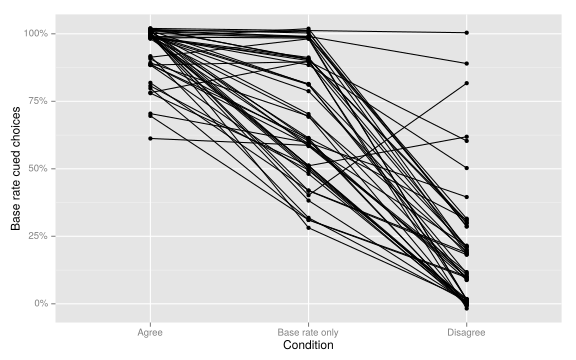
\includegraphics[width=.6\textwidth]{imgs/exp5_br_acc.pdf}
  \caption[Individual differences in the effect of descriptions
  on participants' responses, Experiment 5.]{
    Number of base rate responses per condition, by participant, in Experiment 5.
    \label{fig:exp5_br_acc} }
\end{figure}

\subsubsection{Effect of base rates on description choices}


Base rates had a significant main effect on
the number of description-cued responses given
($\chi^2$  = 67.7, DF = 2, p < .0001).
Pairwise comparisons showed that participants were
less likely to give the description-cued response
when the base rate disagreed with the description (80.4\%)
than when it agreed (94.4\%;
$e^{\beta}$ = 0.20, CI = [0.12, 0.36], z = 6.655, p < .0001)
or when the base rate was uninformative (93.6\%;
$e^{\beta}$ = 0.24, CI = [0.14, 0.42], z = 6.128, p < .0001).
There was no difference between trials in which the base rate agreed
and those where the base rate was uninformative (z < .3, p > .7),
with both conditions close to ceiling.
Therefore, participants were at least in some way
sensitive to the base rate information, and in a minority of cases
relied on it instead of the description when the two conflicted.

Once again, it is useful to investigate individual differences in this effect.
The left panel of Figure~\ref{fig:exp5_description_acc} shows
the proportion of description-cued responses given by each participant by condition.
This shows three participants who were substantially less likely
to give the description-cued response when the base rate disagreed with it.
The right panel shows the difference, for each participant,
in the number of description-cued responses given
from when the base rate agreed to when it disagreed.
This shows that, along with the 
three participants who showed a substantial change,
most participants showed a moderate effect in the same direction:
they were slightly less likely to select
the description-cued response when the base rate disagreed with it,
suggesting that base rates had some effect on the majority of participants.
Out of 50 participants, 28 were less likely
to select the description-cued response when the base rate disagreed,
13 were equally likely to do so (including 10 who always gave this response),
and 9 were actually more likely to select the description-cued response
when the description disagreed.

\begin{figure}[ht]
  \centering
  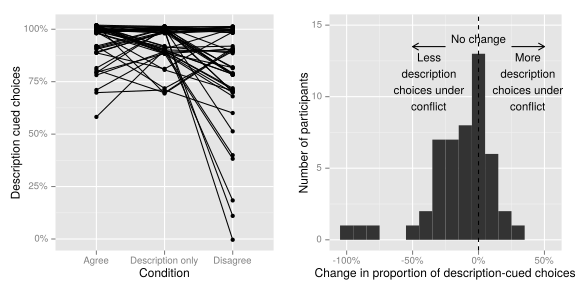
\includegraphics[width=\figurewidth]{imgs/exp5_description_acc.pdf}
  \caption[Individual differences in the effect of base rates
  on participants' responses, Experiment 5.]{
    \label{fig:exp5_description_acc}
    Left: Proportion of base rate-cued responses given in each condition,
    by participant.
    Right: Difference in the proportion of description-cued responses given
    by each participant between when the base rate agreed and disagreed with
    the description. Values below 0 indicate a participant was less likely
    to select the description-cued response when it conflicted with the base rate
    than when it agreed.
  }
\end{figure}



\subsection{Discussion}


 
In this experiment, participants had to generalise a biological property
from a base species to one of two other species:
one that belonged to the same taxonomic group as the base,
and one that did not.
On conflict trials, but not control trials,
there was a strong association between the base and foil,
so participants should have been drawn towards
selecting the foil species on these trials
if this irrelevant associative knowledge plays a role in inductive reasoning.
Replicating the core findings of \citet{Bright},
I found that participants were more likely to select the foil species
on conflict trials,
driven by associative knowledge.

Going beyond previous research, this experiment
allows us to draw inferences about how
these two kinds of knowledge interact.
\citet{Bright} also showed that
participants were more likely to select the foil response under conflict
if they had poor semantic inhibitory control,
or were placed under heavy cognitive load.
This suggests that drawing on the structured knowledge
needed to respond correctly on conflict trials
requires top-down executive functions.
It may be that the actual utilisation of structured knowledge
places demands on these executive processes, or alternatively,
that associative knowledge must be inhibited
before structured knowledge can be retrieved.
Perhaps consistent with the latter interpretation,
I found that on trials where participants did select the correct species,
they were more likely to initially move towards the foil species
on conflict trials, where the foil was strongly associated with the base.

Other findings, however, make this less clear.
The proportion of correct responses that were reversals, for instance,
was low compared to other experiments reported in this thesis:
8\% of control trials, and 16\% of conflict trials.
The current experiment also differed from Experiments 1 and 2
in that participants' response times were no slower
for conflict trials than for control trials.
Similarly, the participants initially moved towards
the foil species on only 35\% of conflict trials,
but after doing so, they only subsequently changed their minds
to select the correct species instead 34\% of the time.
Finally, the time course analysis showed that
even on conflict trials, participants never were more drawn
towards the foil species than the correct one.
Therefore, a more accurate description of these results is as follows.
In some cases participants' mouse movements
were initially driven by associative knowledge,
and later intervened upon on the basis of structured knowledge.
On the majority of conflict trials, however, participants either
moved directly to the species cued by structured knowledge,
or moved straight to the response cued by associative knowledge.

These results differ from those found in Experiments 1 and 2 in a number of ways.
However, before I attempt to interpret these results any further,
a limitation of this experiment must be noted.
Participants' performance on the post-test check,
which was used to ensure that they knew that
each correct response species belonged to the same biological group
as its corresponding base species, was extremely poor.
Specifically, participants' performance was not significantly above chance
when it came to knowing that the following species belonged to the same group:
dolphins and llamas,
monkeys and seals,
snails  and octopuses,
bananas and tulips,
penguins and chickens,
mice and goats,
and Orca whales and cows.
As a result, data from these 7 of the 14 stimuli sets
were excluded from the analysis.
Given that the purpose of this chapter is to study
conflict between associative and structured knowledge,
such poor taxonomic knowledge may be problematic.
Consider, for instance, 
a participant who is drawn towards 
generalising a gene from dolphins to cod,
rather than from dolphins to llamas.
If this participant knows that dolphins and llamas are mammals,
and cod are not, then we can infer that this attraction
is driven by unstructured associative knowledge.
However, if this participant believes that
dolphins and cod belong to the same taxonomic group,
then both their associative and structured knowledge
would support the same inference.
In this case, it is difficult to know what form of knowledge
they are drawing upon.

Therefore, In Experiment 4, I attempted to replicate these findings conceptually,
using new stimuli for which the appropriate taxonomic relationships are more obvious.
Furthermore, Experiment 3 relied on association ratings
collected by \citet[][Chapter 2]{Crisp-Bright2010}
from a different pool of university students,
and only allowed for the manipulation of the foil species,
which was either strongly associated with the base,
according to the prior ratings,
or (assumed to be) not associated.
In Experiment 4, in contrast,
I collected association ratings for each species pair
from each participant, after they had completed the rest of the experiment.
In this way, it was possible both to
investigate the relationship between association ratings
and participants' choices and cursor movements in a more nuanced way,
and to use each participants' actual beliefs about
the strength of association between species,
rather than aggregate ratings from a separate pool of participants,
in the analyses.


\section{Experiment 4}

In Experiment 4, I attempted to replicate the findings of Experiment 3,
but without the need to discard data from
trials for which participants lacked appropriate taxonomic knowledge.
Beyond this, I wished to explore
how each participants' own beliefs about the strength of association
between various species interacted with structured knowledge during reasoning.
Therefore, in this experiment, I asked participants to rate
the association between each base species
and every response species it was paired with for the reasoning trials.
This improves on the method used in the previous study in two ways.
First, while \citet[Chapter 2]{Crisp-Bright2010} collected
ratings of the association between the base species,
the correct response species, and the strongly associated foils used in the previous experiment,
she did not collect ratings for the associations between the bases
and the foil species assumed to be weakly associated.
Second, \citet{Crisp-Bright2010} collected
association ratings from one set of participants,
and reasoning data from another.
Therefore, it was the average association rating between species
that she used as a predictor in here analyses.
Here, on the other hand, I collected each participants'
own idiosyncratic ratings of the associations between the species,
allowing a more fine-grained analysis of
how such associative knowledge influences reasoning.


\subsection{Method}

\subsubsection{Participants}

Forty four undergraduate students completed the experiment
in exchange for course credit, in a laboratory.
The experiment was programmed using the OpenSesame experiment builder
(see Chapter 2).

\subsubsection{Stimuli}

In the experimental trials, participants were asked about
biological properties, specifically cells.
Nine new stimulus sets were generated for the experimental trials,
intended to be more familiar to participants
than those used in Experiment 3.
Each new set had three foil species,
one intended to be weakly, one moderately,
and one strongly associated with the base.
Each set was presented three times, once with each foil species.
Stimuli were selected according to a number of partial pretests,
in which participants rated the strength of association between species
using the procedure from \citet[][Chapter 2]{Crisp-Bright2010}, described above.
The full set of stimuli can be found in Appendix~\ref{appendix:exp4_stimuli}.

For the filler trials, where participants were asked about diseases,
an additional fourteen stimulus sets were generated,
each containing a base species,
a correct response species likely to share a disease with the base,
and three different foil responses, one for each time the set was presented.
One possible concern about the design of Experiment 3
is that the species designated as the correct response
for each experimental stimulus set
was the correct response on every trial it featured in.
Therefore, the fourteen correct response species from the experimental trials here
were used as foil species (that is, the species that
were unlikely to share a disease with the base species)
on three different filler trials.
This meant that these species were the correct response option
in the three experimental trials in which they featured,
but also the incorrect response option in three filler trials.
The properties to be reasoned about ---
genes on the experimental trials,
and diseases on filler trials~---
were unchanged from Experiment 3.

To ensure that participants did not complete
experimental trials with the same base species in close succession,
the order of trials was randomised with constraints for each participant.
First, the experimental trials were randomly divided
into three blocks of nine trials,
with each block containing
three weak, three moderate, and three strong foils,
and one trial from each stimulus set in each.
Nine of the twenty-seven filler trials were then added to each block.
Finally, the order of trials within each block was randomised repeatedly,
until at least 5 trials separated repetitions of each base species.

\subsubsection{Procedure}

There were minimal changes to the reasoning trials from Experiment 3.
However, this experiment was conducted using the OpenSesame platform,
which allowed greater experimental control over the mouse cursor.
Therefore, instead of requiring participants
not to move the cursor during the fixation period,
the cursor's position was automatically reset
to the centre of the START button after the fixation.

After the reasoning trials, participants again completed a post-test check.
In the first part of the post-test, participants rated the strength of association
of the thirty-six base-response species pairs from the experimental trials.
These consisted of the nine base species,
each of which was paired with its correct response species
and its three foil species.
For this section, participants were presented with the following instructions,
taken directly from  \citet[][Chapter 2, p. 60]{Crisp-Bright2010}:

\begin{quote}
  [...] Please think about all kinds of possible associations, such as causal,
  functional, categorical, etcetera. Please do not think in detail about
  the mechanism by which they are related, just give your intuitive
  response. For example, if you believe that ladybirds and butterflies
  are strongly associated please give a rating closer to 9. In contrast,
  if you think cars and ladybirds are unrelated, please give a rating
  closer to 1. Please give the answer that first comes to mind, as fast
  as possible.  
\end{quote}

On each rating trial, the labelled images of each species
were shown side by side, with their positions randomised.
Participants gave their ratings by clicking on buttons
labelled 1 to 9 below the images,
with 1 subtitled ``Not associated at all'',
and 9 subtitled ``Very strongly associated''.

The second part of the post-test checked participants' structured knowledge.
Participants were presented with pairs of species,
in the same format as the association rating trials,
and gave yes or no responses by clicking the marked buttons.
There were three blocks in this part of the post-test,
and the order of trials within each block was randomised.
First, for each of the nine experimental stimulus sets,
the base species and the correct response species
belonged to the same taxonomic group.
These nine pairs of species were presented along with
an additional nine pairs that did not belong to the same group.
Participants were asked in each case if the pair shown
belonged to the same \emph{biological group}, and told
``Biological groups are the main branches
when you think about the `family tree' of the natural world'',
and that the biological groups in the experiment were
mammals, fish, reptiles, birds, and plants.

Second, for five of the experimental stimulus sets,
the base species was related to the moderately and strongly associated foils
via a food chain relationship --- one species eats the other.
These ten base-foil pairs were presented along with
ten other species pairs not related in this way.
Participants were asked if each pair shown belonged to the same \emph{food chain},
and told ``Species belong to the same food chain if one is eaten by the other
(predators and prey for animals, or a plant which is eaten by an animal)''.

Finally, for the remaining four experimental stimulus sets,
the base species was related to the moderate and strong foils
in that they shared an ecological habitat.%
\footnote{
  This was not technically true for penguins and arctic wolves,
  and penguins and polar bears, as these species live in
  opposite polar regions, but the post-test data showed that
  participants do not realise this.
}
These eight base-foil pairs were presented along with
the eight other pairs that did not share a habitat,
and participants were asked if thee pair shown ``live in the same kind of habitat''.



%%% Local Variables: ***

\subsection{Results}

\subsubsection{Post Test Check}

For each stimulus set used in the experiment,
participants correctly said that the base species
and the correct response species 
belonged to the same taxonomic group (accuracy > 70.5\%, p's < .01),
and that the moderate and strong foils
had the appropriate relationship (food chain or shared habitat)
with their base species (accuracy > 75\%, p's < .001).
Therefore, no data were excluded from the analyses on these criteria.
Full post-test results can be found in Appendix~\ref{appendix:exp4_posttest}.

\subsubsection{Reasoning Accuracy}

In order to analyse data from the reasoning trials,
for each trial I divided that participants' rating of
the association between the base and the correct species
by their rating of the association between the base and the foil.
This produced a ratio reflecting the extent to which
that participants' associative knowledge
favoured one or other response option.
Values of this ratio ranged from $\frac{1}{9}$
($.111$; association of 1 for the correct species, and 9 for the foil),
to $\frac{1}{1}$ (equal association for both species),
to $\frac{9}{1}$
(association of 9 for the correct species, and 1 for the foil).

For each analysis, I log-transformed this ratio
to create a normally-distributed linear predictor,
as is standard practice when using ratios as regression predictors \citep{Gelman2007}.
Note that $log(\frac{1}{1}) = 0$,
and correspondingly $log(\frac{>1}{1}) > 0$ and $log(\frac{1}{>1}) < 0$
(see Figure~\ref{fig:exp4_log_transform}).
Therefore, when using the log-transformed ratio as a predictor,
a positive regression weight means that
the dependent variable is greater/more likely when the ratio is greater than $\frac{1}{1}$,
or in other words, when the association rating favours the correct response.

\begin{figure}[h]
  \centering
  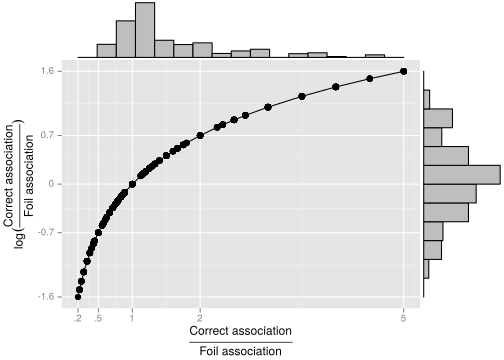
\includegraphics[width=.7\textwidth]{imgs/exp4_log_transform.pdf}
  \caption[The log-transformed association ratio, used as a predictor in Experiment 4.]{
    To analyse data from Experiment 4,
    each participants' rating for the association between
    the base species and the correct response species
    was divided by their rating for
    the base and the foil species, to form an association ratio.
    These ratios were log-transformed to use as predictors in regression analyses:
    after log-transformation, the difference between 1 and 0.2 (dividing by five)
    is the same as the difference between 1 and 5 (multiplying by five).
    \label{fig:exp4_log_transform}
  }
\end{figure}

Some aspects of the analyses based on this ratio are slightly unusual,
and so I will go through my first analysis,
predicting participants' responses,
in detail to familiarise readers with the method.
Figure~\ref{fig:exp4_ratio_accuracy} plots the proportion of correct responses 
(choosing the species belonging to the same taxonomic group as the base) given, on the y axis,
as a function of the association ratio, on the x axis.
Note that the x axis is log-scaled.
For plotting, I have divided the log-transformed ratio into 13 equal bins,
and plotted the mean and standard error of the dependent variable within each bin.
For the analyses, I fit log-linear, or logistic mixed models,
with random intercepts for each participant, and for each stimulus set.
The log-transformed association ratio from each trial was used as the predictor in the models.

\begin{figure}[h]
  \centering
  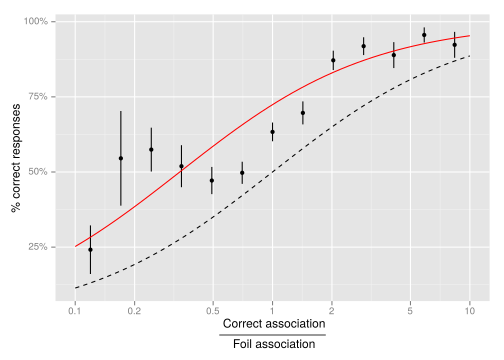
\includegraphics[width=.6\textwidth]{imgs/exp4_ratio_accuracy.pdf}
  \caption[Effect of the association ratio of participants' accuracy, Experiment 4.]{
    Correct responses on Experiment 4, as a function of
    the association ratio in favour of the correct species.
    As the ratio increased in favour of the correct species,
    participants became more likely to select that species.
    The fitted model (red line) included a significant positive intercept term,
    meaning that participants were more likely to select the correct species
    than would be predicted based on the association ratio alone (dashed black line).
    \label{fig:exp4_ratio_accuracy}
  }
\end{figure}

The association ratio was a significant predictor of the odds of a correct response
($\beta$ = 0.89, CI = [0.68, 1.1], z = 8.604, p < .0001).
Interpretation of the regression $\beta$ here is not straightforward,
but positive $\beta$s indicate that the dependent variable
(odds of a correct response) was positively related to
the size of the association ratio in favour of the correct response.
Fortunately, we can simply look to the predicted values from this model
(solid red line in Figure~\ref{fig:exp4_ratio_accuracy})
to see the magnitude of this effect.

An unusual property of these models is that
the intercept parameter is also meaningful.
As the log-transformed association ratio is the only predictor in the model,
the intercept reflects the expected value
when this predictor is at 0, or in other words, for a ratio of $\frac{1}{1}$.
If participants do not make use of structured knowledge,
we would expect participants to select the correct species
50\% of the time for such trials, something that would correspond to an intercept of 0.
The dashed black line in Figure~\ref{fig:exp4_ratio_accuracy}
shows the predicted values for such a model, with intercept 0.
A significant positive intercept means that
participants were more likely to select the correct species
than would be expected from the association ratio alone,
while a negative intercept means they were less likely.
There was a significant positive intercept term in this model
($logit(\beta)$ = 72\%, CI = [56\%, 85\%], z = 2.585, p = .0010).
I report the $logit$ of the regression $\beta$ weights here
as an easily interpretable measure of how much participants
were biased towards the correct species.
In this case, $logit(\beta)$ reflects how often
participants would be expected to select the correct species
on trials where the association ratio = $\frac{1}{1}$,
according to the fitted model
(i.e. where the red line on Figure~\ref{fig:exp4_ratio_accuracy}
crosses $1$ on the x axis).
Together, these results mean that participants were
a) more likely to select the correct species when
they rated it as being more strongly associated with the base
than the foil was, and
b) biased towards the correct option rather than the foil
beyond the effect of the association ratio.

\begin{figure}[h]
  \centering
  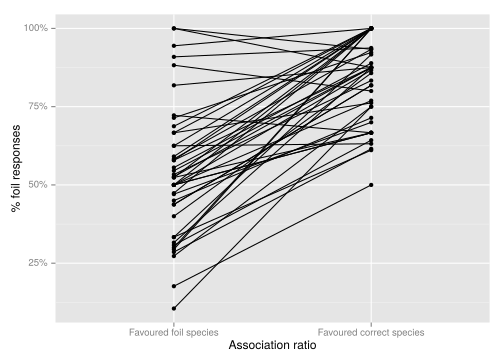
\includegraphics[width=.7\textwidth]{imgs/exp4_acc_ids.pdf}
  \caption[Proportion of correct responses
    given by each participant, by association ratio,
    in Experiment 4]{
    Participants' number of correct responses
    on trials where the association ratio favoured either
    the correct species or the foil species.
    40 of 44 participants were more likely to select the correct species
    when the association ratio favoured it
    than when the ratio favoured the foil.
    \label{fig:exp4_acc_ids} }
\end{figure}

To analyse individual differences in the number of correct responses
(Figure~\ref{fig:exp4_acc_ids}),
I calculated the number of correct responses given by each participant
both when the association ratio favoured the foil species,
and when it favoured the correct species,
excluding trials where species were rated as equally associated.
Of the 44 participants, 40 were more likely to select the correct species
when the association ratio favoured it,
and 4 were less likely to do so.
Therefore, it appears that almost all of my participants
were influenced by the association between species.

\FloatBarrier
\subsubsection{Correct Responses}

Analysing trials where the correct species was selected,
the association ratio had no effect on participants' movement initiation times
(mean = 574 msec, SD = 285; t(529.6) = 0.387, p > .6).
There was a marginally significant effect of the association ratio
on participants' response latencies
(mean RT = 1509, SD = 567;
$e^{\beta}$ = 98\%, CI = [96\%, 100.4\%], t(787.1) = 1.647, p =.100),
meaning that participants were marginally faster to respond correctly
as the association ratio in favour of the correct species increased.

Maximum deviation was once again bimodally distributed
(Bimodality Coefficient = .635; Hartigan's D = .025, N = 1188, p < .0001),
and reversal trajectories were classified
as described in Chapter 2 (MD cut-off = 0.923, see Appendix~\ref{appendix:reversals}).
Figure~\ref{fig:exp4_reversals} shows the proportion of correct responses
that were categorised as reversals ---
that is, where participants moved initially towards the foil
before selecting the correct species ---
as a function of the association ratio.
A logistic mixed model (dashed red line) showed that
participants were less likely to follow such a reversal trajectory
as the association ratio increased in favour of the correct species
($e^{\beta}$ = .8, CI = [.6, .97], z = 2.152, p = .0314).
However, the data were fit slightly better%
\footnote{
  As these two models were not nested,
  and contained the same number of parameters,
  we can identify which model best fits the data
  by comparing the deviance of each,
  but we cannot calculate p values for
  the difference between the models.
}
($\Delta$deviance = $0.715$)
by an alternative model (solid red line),
where the odds of a trajectory being classed as a reversal
when selecting the correct species
were predicted by the \emph{absolute magnitude} of the log-transformed association ratios
($e^{\beta}$ = .7, CI = [.5, .9], z = 2.289, p = .0221).
In other words, when selecting the correct species,
participants were most likely to trace a reversal trajectory
when the species were equally associated,
and less likely to do so as the ratio changed in favour of either species.
This trend may appear counter-intuitive,
but may make sense when one considers that
this analysis does not include trials where the foil species was selected.
An explanation for the trend is offered in the discussion, below.


\subsubsection{Cursor Trajectories}


As before, mouse trajectories in this experiment
can be described in terms of whether or not
they initially moved towards the correct species ($\alpha$),
whether they selected the correct species
after initially moving towards it ($\beta$),
and whether they changed direction to select the correct species
after initially moving towards the foil ($\gamma$;
see Figure~\ref{fig:exp3_transitions}).
I modelled these three parameters
using multilevel logistic regression models,
with the log-transformed association ratio
and an intercept term as predictors,
and random intercepts for each participant and stimulus set.

\begin{figure}[tp]
  \centering
  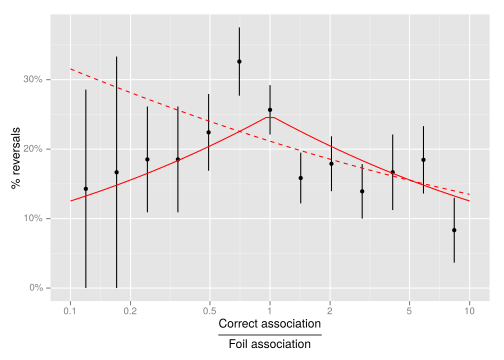
\includegraphics[width=.7\textwidth]{imgs/exp4_reversals.pdf}
  \caption[Proportion of correct responses that involved reversals,
  Experiment 4.]{
    The proportion of correct responses
    where participants initially moved towards the foil species.
    A model using the log-transformed association ratio as a predictor
    (dashed red line) showed that participants were more likely
    to produce these reversal trajectories when the association ratio
    favoured the foil species.
    However, the data were slightly better fit by a model (solid red line)
    which showed that these reversals were most likely to occur
    when the association ratio favoured neither response.
    \label{fig:exp4_reversals}
  }
\end{figure}

\begin{figure}[bp]
  \centering
  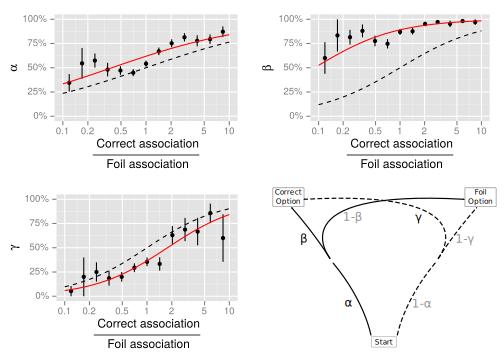
\includegraphics[width=.7\textwidth]{imgs/exp4_transitions_combined.pdf}
  \caption[Transition probabilities, as a function of the association ratio,
    in Experiment 4.]{
    \label{fig:exp4_transitions}
    Transitions probabilities from Experiment 4,
    as functions of the association ratios.
    As the association ratio increased in favour of the correct species,
    participants became more likely to initially move towards that species ($\alpha$, top left),
    to select that species after initially moving towards it ($\beta$, top right),
    and to select it even after initially moving towards the foil ($\gamma$, bottom left).
    Dashed lines show the expected values if participants were
    influenced by association ratio only.
    Overview of the three parameters can be seen in the bottom right.
  }
\end{figure}


The model for $\alpha$ (Figure~\ref{fig:exp4_transitions}, top left)
had a marginally significant positive intercept
($logit(\beta)$ = 62\%, CI = [50\%, 73\%], z = 1.886, p = .0593)
indicating that participants initially moved towards the correct species
on 62\% of trials when the ratio was $\frac{1}{1}$,
more than the 50\% that would be expected 
based on the association ratio alone.
The association ratio was also a significant positive predictor
($e^{\beta}$ = 1.7, CI = [1.4, 2.0], z = 6.109, p < .0001)
such that participants became more likely to initially move
towards the correct species as it was increasingly favoured by the association ratio.

The model for $\beta$  (Figure~\ref{fig:exp4_transitions}, top right)
had a robust positive intercept
($logit(\beta)$ = 80\%, CI = [85\%, 92\%], z = 10.567, p < .0001),
meaning that after initially moving towards the correct species,
participants selected that species 80\% of the time
when the association ratio was $\frac{1}{1}$.
The association ratio was also a significant positive predictor here
($e^{\beta}$ = 2.4, CI = [1.8, 3.2], z = 5.678, p < .0001),
meaning that participants became more likely to select the correct species
on trials where they initially moved towards it
as the association ratio in favour of the correct species increased.
In general, however, participants very rarely
changed direction after moving towards the correct species
in any case.

Finally, the model for $\gamma$  (Figure~\ref{fig:exp4_transitions}, bottom left)
contained a significant \emph{negative} intercept
($logit(\beta)$ = 37\%, CI = [30\%, 43\%], z = 3.963, p < .0001),
indicating that on trials where they initially moved towards the foil species,
participants only changed direction to select the correct species instead
37\% of the time when the association ratio was $\frac{1}{1}$.
The association ratio was again a positive predictor here
($e^{\beta}$ = 2.6, CI = [2.0, 3.5], z = 6.374, p < .0001),
meaning that as the strength of the association ratio
in favour of the correct species increased,
participants were more likely to switch direction
and select the correct species when they initially moved towards the foil.


\subsubsection{Time course}
\FloatBarrier

\begin{figure}[ht]
  \centering
  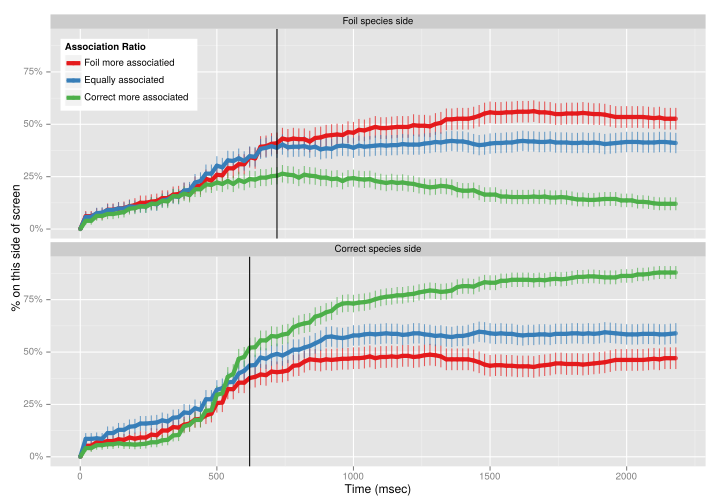
\includegraphics[width=\figurewidth]{imgs/exp4_condition_timecourse.pdf}
  \caption[Time course, separately for each response option, in Experiment 4.]{
    Proportion of trials on side of screen corresponding to the correct species (top)
    and the foil species (bottom) over time.
    The association ratio is a significant predictor
    of movements towards the foil from 720 msec,
    and of movements towards the correct species from 620 msec (solid vertical lines).
    \label{fig:exp4_condition_timecourse} }
\end{figure}


As usual, the time course of  the mouse movements here
reveals more about the points at which participants were
drawn towards each response.
Figure~\ref{fig:exp4_condition_timecourse} shows the proportion of trials
on the side of the screen corresponding to each species over time,
for trials where the association ratio favours the foil species (N = 359),
the two species were rated as equally associated (N = 397),
or the correct species was more strongly associated (N = 432).
To estimate divergence times,
I fitted two series of logistic mixed models,
one series predicting the probability of being on the foil species' side of the screen,
and one the probability of being on the correct species' side,
separately for every 20 msec time window.
Each model included the log-transformed association ratio  as a predictor,
and included random intercepts for each participant and each base species.
The divergence points were the times in each series
after which the association ratio is found to be a significant predictor.
The association ratio had a significant effect on
participants' probability of being on the foil species'
side of the screen from 720 msec,
and their probability of being on the correct species' side from 620 msec.

\begin{figure}[h]
  \centering
  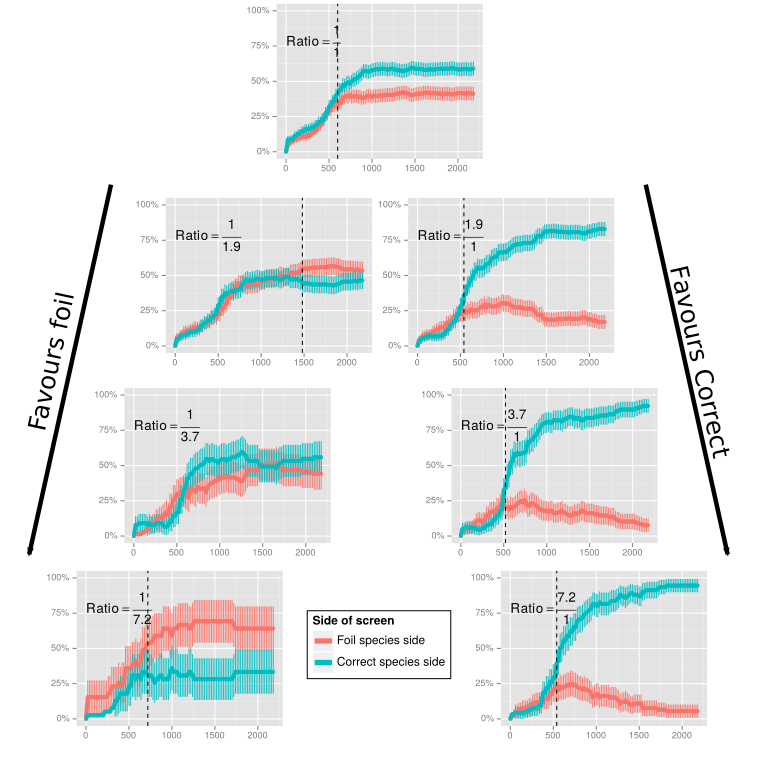
\includegraphics[width=\figurewidth]{imgs/exp4_ratio_timecourse.pdf}
  \caption[Time course, separately for different association ratios, in Experiment 4.]{
    Proportion of trials on the side of the screen corresponding to each response,
    grouped by association ratios.
    When the association ratio favours the correct option,
    %% \aside{This figure should have the divergence points marked for each trial,
    %%   a legend somewhere, and the font sizes all the same.
    %%   I will do this in the next few days when I've the use of a computer with a mouse.}
    \label{fig:exp4_ratio_timecourse} }
\end{figure}

\begin{table}
  \centering
  \caption[Divergence times, Experiment 4.]{
    Divergence times, and number of trials included,
    for each binned value of the association ratio.
    For ratios of $\frac{1}{7.2}$ and $\frac{1}{1.9}$,
    participants were significantly more likely to be on
    the foil species' side of the screen than the correct species'
    from the divergence time onwards.
    For all other ratios, participants were more likely to be on
    the correct species' side of the screen
    from the divergence time.
    \label{tab:exp4_ratio_timecourse_table}
  }
  \doublespacing
  \begin{tabular}{lrr}
    \toprule
    Ratio           & Divergence (msec) & N\\
    \midrule
    $\frac{1}{7.2}$ & 720               & 39\\
    $\frac{1}{3.7}$ & N/A               & 77\\
    $\frac{1}{1.9}$ & 1,480              & 243\\
    $\frac{1}{1}$   & 600               & 397\\
    $\frac{1.9}{1}$ & 540               & 223\\
    $\frac{3.7}{1}$ & 520               & 117\\
    $\frac{7.2}{1}$ & 540               & 92\\
    \bottomrule
  \end{tabular}
\end{table}

Figure~\ref{fig:exp4_ratio_timecourse}
shows the proportion of trials on either side of the screen,
with separate plots representing different levels of the association ratio.
For this analysis, I divided the log-transformed association ratio
into seven bins of equal width,
and labelled each bin according to the mean association ratio within it:
$\frac{1}{7.2}$, $\frac{1}{3.7}$, $\frac{1}{1.9}$, $\frac{1}{1}$, $  \frac{1.9}{1}$, $\frac{3.7}{1}$, and $\frac{7.2}{1}$.
Within each of these bins, I found the divergence point,
after which participants were more likely to be
on one side of the screen than the other,
by fitting a series of logistic mixed models,
comparing the probability of being on either side of the screen,
with random intercepts for each participant and each base species.

As the association ratio in favour of the correct species increased,
from $\frac{1}{1}$ (both species equally associated) up to $\frac{7.2}{1}$
(correct species 7.2 times more strongly associated than the foil),
we see a clear increase in the number of trials where
the cursor ends up on the correct species' side,
mirroring the earlier analysis of participants' responses.
There was little difference, however,
in the trends leading up to these final proportions.
For all of these bins, the preference for the correct species
emerged from 520 -- 600 msec,
and the shape of the curves were broadly similar,
except for the differences in their overall heights.
Thus, structured knowledge began to influence
participants' motor output from \tildetext600 msec.

When the association ratio was less than $\frac{1}{1}$, however,
and so conflicted with structured knowledge,
the trends were less clear.
When the ratio was strongest in favour of the foil species ($\frac{1}{7.2}$),
participants were more likely to move towards the foil
than the correct species from 720 msec.
Both species were equally attractive with a ratio $\frac{1}{3.7}$, however,
and with a ratio of $\frac{1}{1.9}$ a significant preference for the foil
only emerged from 1,480 msec.
Note, however, that even when the association ratio
conflicts with structured knowledge,
there is no evidence of a cross-over relationship ---
in each subplot within Figure~\ref{fig:exp4_ratio_timecourse},
participants were either drawn to the correct species, or to the foil,
but in no case were they primarily initially drawn towards the foil,
and later drawn towards the correct species.




\subsection{Discussion}

In general, the results of this experiment
are consistent with Experiment 3,
but unlike in Experiment 3, I did not exclude any data
on the basis of the post-test results.
Participants' inferences were influenced by both
associative and structured knowledge.
Associative knowledge was indexed by the association ratio,
reflecting how strongly each participant rated
the association between the base and the correct species,
compared to the base and the foil.
This was a strong predictor of their inferences,
with participants more likely to project the property
to the correct species as its association with the base increased,
relative to the foil.
If participants only relied on associative knowledge, however,
they should give the correct response only 50\% of the time
when the association ratio favoured each response equally (ratio of $\frac{1}{1}$).
In reality, the fitted model predicted 72\% accuracy on such trials,
indicating that participants were also influenced
by structured taxonomic relationships.

Unlike Experiment 3, the current experiment revealed
that response times for correct responses were
marginally faster when the association ratio favoured the correct species
(i.e. when the associative and structured knowledge cued the same response).
There were, however, faster movement initiation times
for conflict trials in Experiment 3,
a finding that was not replicated here.
Of course, these two results are likely related:
initiation times are included in total response times,
and so faster initiation times under conflict in the previous experiment
may cancel out an overall effect on response time.
However, my analyses do not rest on these measures,
and so I will not attempt to interpret them further.

More interesting are the analyses of the cursor trajectories.
First, I found that initial cursor movements
were strongly predicted by associative knowledge,
and only marginally predicted by structured knowledge:
strength of association being equal,
participants are expected to move towards the correct species 62\% of the time.
After moving towards the correct species,
participants rarely
(20\% of the time when the species were equally associated)
changed direction to select the foil instead,
although they were more likely to do this
if the foil was more strongly associated than the correct species.
After initially moving towards the foil species, however,
participants were somewhat more likely to change direction:
they were predicted to do so 37\% of the time
when the association strengths were equal,
and more often when the correct species was more strongly associated.

From all of this, we can conclude three things.
First, associative knowledge predicts participants' movements
at every possible juncture, and unsurprisingly,
participants are more drawn towards a response option
when it is more strongly associated than the alternative.
Second, structured knowledge also plays a role at every juncture.
Participants were marginally more likely
to initially move towards the correct species
than would be expected based on associative knowledge alone,
and later, participants were in general more likely to change direction
to the correct species after initially moving towards the foil (37\%)
than to change to the foil species after
initially moving towards the correct one (20\%).
Third, once they started moving towards a response option,
participants in this experiment were unlikely to change direction.

Analysing the proportion of correct responses
where the cursor trajectory was classified as a reversal,
an unexpected trend emerged.
The data could be modelled using the association ratio as a predictor:
correct responses were more likely to involve
initial movements towards the foil
when the foil was more strongly associated than the correct species.
However, the data were slightly better fit by a model that
used the magnitude of this ratio
(how far it was from a ratio of $\frac{1}{1}$, in either direction),
resulting in the inverted U trend seen in Figure~\ref{fig:exp4_reversals}.

However, while this pattern was unexpected,
it can be understood in light of the transition probabilities, discussed above.
Participants were, first of all, more likely to
initially move towards the correct species
when the association ratio favoured this response.
Additionally, regardless of their initial movement,
participants were also more likely to ultimately select the correct species
when it was favoured by the association ratio.
Combined, these factors produce three kinds of trajectory.
When the association ratio strongly favoured the correct species,
participants moved straight towards that species, and selected it,
rarely moving to the foil at all,  and yielding few reversals.
When the ratio favoured the foil species,
participants who moved towards the foil usually ended up selecting it,
leaving few who moved to the foil before selecting the correct species.
When the ratio did not favour either species, however,
some participants  moved towards the foil initially,
and some of these changed their minds,
yielding a higher number of reversal trajectories.

Finally, the time course trends here are consistent with those found in Experiment 3.
As the association ratio becomes stronger in favour of the correct species,
participants became more likely to ultimately select this species,
but there were no striking changes in the trends leading up to these responses.
Additionally, consistent with the analysis of the transition probabilities,
even when associative and structured knowledge conflicted strongly,
there was no indication that participants were
first driven by associative knowledge,
and then by structured knowledge.
This is again consistent with the trends seen for Experiment 3.




\section{General Discussion}


In these two experiments
participants completed versions of the inductive triad task
where they were asked to generalise a property from a base category
to one or other response category.
They could rely either on conceptual knowledge,
and so generalise the property to the category that
belonged to the same category as the base,
or on perceptual cues,
and generalise to the category that looked like the base.
In both experiments, I manipulated whether the cues agreed or disagreed,
so that on conflict trials perceptual cues would lead participants
to select the foil response option rather than the
conceptually-related one.
On these conflict trials, participants were
more likely to select the foil category.
Furthermore, they were more likely to make
fast initial mouse movements towards the foil,
which they often overrode to select the correct category instead.
These results are consistent with \citegap{Bright2014a}{'s} hybrid theory of induction.

I also raised the question of how perceptual cues
and conceptual knowledge might interact during induction.
One option was that participants
selectively relied on perceptual cues \emph{or} conceptual knowledge.
The alternative was that participants were
initially driven by perceptual cues,
but sometimes overrode theses cues when they realised them to be inappropriate,
and relied on conceptual knowledge instead.

The results showed that participants,
although usually initially moving towards the perceptually-cued foil,
sometimes moved directly towards the conceptually-cued option,
with these movements generally taking longer to initiate
than those towards the foil.
There are two possible explanations for such trials.
It may be that participants simply draw on conceptual knowledge here,
a process which takes longer, and then act on it.
Alternatively, participants on these trials
may have first processed the perceptual cues,
but inhibited them and replaced them with their conceptual knowledge
before initiating their cursor movement.
It is not clear at present how these possibilities could be disentangled,
and so for the time being this particular issue remains an open question.

In Experiment 2, I manipulated the kinds of properties participants reasoned about:
either specific properties, that were saliently related
to the distinction between the two categories,
or generic properties, that were not.
This manipulation mainly affected what participants did
on trials where they initially moved towards a perceptually-cued foil option.
Participants reasoning about specific properties were
significantly more likely to override their initial movement
and select the correct option instead
than those reasoning about generic properties.
The manipulation did not make participants any less likely
to initially move towards the foil option,
and its influence on the time course data
emerged relatively late in reasoning (see Figure~\ref{fig:exp2_foil_side_timecourse}).
It also had no influence on control trials,
where participants almost invariably selected the correct option.
Therefore, it would appear that this manipulation
mainly served to make participants more likely
to inhibit their perceptually-driven responses
on trials in which they were initially driven towards giving them.
This is consistent with much previous work,
both using the current paradigm \citep{Gelman2013c}
and other inductive tasks \citep{Heit1994,Ross1999},
indicating that the kind of information people draw on in inductive reasoning
is contingent on the nature of the properties to be projected.
A future question raised by this result concerns
whether this manipulation serves to make
participants more likely to inhibit perceptual cues,
or if it makes certain structured knowledge
easier to retrieve by cuing or priming it.

The purpose of these experiments
was to investigate adults' inductive reasoning,
and the results are consistent with \citegap{Bright2014a}{'s} hybrid account.
Specifically, they suggest that induction cannot be explained entirely
by either accounts based on unstructured associative knowledge
such as (perceptual or representational) similarity
\citep[i.e.][]{Sloman1993,Rogers2004,Sloutsky2004,Fisher2015}
or by purely structured, conceptual knowledge
\citep[i.e.][]{Osherson1990,Griffiths2009,Kemp2009,Gelman1986}.
Instead, both kinds of information appear to influence adults' reasoning,
with simple perceptual similarity drawn on earlier in the process,
and perhaps serving as a default.
However, these results also have implications for theories of children's reasoning.
As discussed in Chapter 1, and earlier in the current chapter,
a number of experiments have claimed to show that
young children's inferences are either
driven by conceptual knowledge
\citep{Gelman2013c,Rhodes2009,Gelman2007a,Gelman1986},
or that they are driven by perceptual similarity
\citep{Sloutsky2008,Sloutsky2007,Sloutsky2004a}.
These previous experiments \citep[i.e.][]{Gelman1986,Sloutsky2007,Gelman2013c},
however, have focused on a binary question:
do children draw on perceptual cues, \emph{or} on conceptual knowledge during reasoning?
Therefore, these experiments only presented participants with conflict trials,
and their responses were classed as either
consistent with reliance on perceptual similarity,
consistent with reliance on conceptual knowledge,
or not significantly different from chance in either direction.
As discussed in Chapter 1,
an experimental control condition, of the type used here,
where both cues agree, makes it possible to discover
not only which cue dominates when both conflict,
but also whether the neglected cue,
perceptual similarity in this case,
has any influence at all.

Therefore, these results with adults suggest a new interpretation
of the developmental data:
if both perceptual similarity and conceptual knowledge influence adults' reasoning,
they likely both also play a role in children's inferences.
This perspective may make sense of
apparently contradictory results in the developmental literature,
where children seem to draw on conceptual knowledge
in some scenarios but not others.
It is likely that these studies differ
in terms of the factors which make participants
more or less likely to inhibit initially influential perceptual cues.
Thus, while children may have access to both perceptual cues
and information about conceptual knowledge across all of these experiments,
they are more likely to inhibit the former in favour of the latter
when categories differ at a high, ontological level,
when entities are more easily categorised,
or when the properties under consideration are
conceptually related to the distinction between the categories
\citep{Gelman2013c}.
In short, the current results suggest that
developmental researchers should be less concerned
about \emph{whether} children rely on similarity or on conceptual knowledge,
and instead ask \emph{when} do children rely on either form of information.



% \aside{ This is where Newall 20 questions with nature bit comes in! }







% Having shown that perceptual and conceptual knowledge
% are activated during induction,
% our next question is how to these representations
% interact during the reasoning process.
% \aside{I need to look at trajectories when the wrong response was chosen.}
% Unlike a number of mouse tracking studies
% that found graded, continuous attraction towards both responses \citep[i.e.][]{Spivey2005},
% we found that participants moved directly towards one or other response,
% and on many trials moved initially towards one, before changing direction mid-flight.
% Earlier trajectories were more likely to be directed
% towards the perceptually-cued response option
% while later movements moved towards the conceptually-related option.
% This is consistent with the idea that only one representation
% can exist in working memory at a time.










\begin{appendices}
  %% \setcounter{secnumdepth}{0}
  \appendixpage
  \graphicspath{{./../Appendices/}}
  
  \chapter{Stimuli from Experiment 1}\label{appendix:exp1_stimuli}
    %% http://tex.stackexchange.com/a/88939/60964
  % \centering
  %%   \hspace*{-2cm} \begin{tabular}{rcccc}
  %%   \toprule
  %%   Set & Base species                     & Correct option                & Conflict foil                 & Control foil \\
  %%   \midrule
  %%   1   & \smallpic{imgs/bird}             & \smallpic{imgs/flamingo}      & \smallpic{imgs/bat}           & \smallpic{imgs/fox}          \\
  %%   2   & \smallpic{imgs/dandelions}       & \smallpic{imgs/roses}         & \smallpic{imgs/coral_flower}  & \smallpic{imgs/coral_brain}  \\
  %%   3   & \smallpic{imgs/bug_leafy}        & \smallpic{imgs/bug_ladybird}  & \smallpic{imgs/plant_leaf}    & \smallpic{imgs/tree_winter}  \\
  %%   4   & \smallpic{imgs/hedgehog}         & \smallpic{imgs/dog}           & \smallpic{imgs/pinecone}      & \smallpic{imgs/sycamore}     \\
  %%   5   & \smallpic{imgs/dino_triceratops} & \smallpic{imgs/dino_sauropod} & \smallpic{imgs/rhino}         & \smallpic{imgs/cat}          \\
  %%   \bottomrule
  %% \end{tabular}\hspace*{-2cm}
  \vspace*{-2cm}\begin{longtable}{rcccc}
    \caption[]{ Stimulus images used in Experiment 1.} \label{} \\
    
    \toprule
    Set & Base species                     & Correct option                & Conflict foil                 & Control foil \\
    \midrule
    \endfirsthead

    \toprule
    Set & Base species                     & Correct option                & Conflict foil                 & Control foil \\
    \midrule
    \endhead

    %% \hline \multicolumn{3}{|r|}{{Continued on next page}} \\ \hline
    \bottomrule
    \endfoot
    
    \bottomrule
    \bottomrule
    \endlastfoot

    1   & \smallpic{imgs/exp1/bird}             & \smallpic{imgs/exp1/flamingo}      & \smallpic{imgs/exp1/bat}           & \smallpic{imgs/exp1/fox}          \\
    2   & \smallpic{imgs/exp1/dandelions}       & \smallpic{imgs/exp1/roses}         & \smallpic{imgs/exp1/coral_flower}  & \smallpic{imgs/exp1/coral_brain}  \\
    3   & \smallpic{imgs/exp1/bug_leafy}        & \smallpic{imgs/exp1/bug_ladybird}  & \smallpic{imgs/exp1/plant_leaf}    & \smallpic{imgs/exp1/tree_winter}  \\
    4   & \smallpic{imgs/exp1/hedgehog}         & \smallpic{imgs/exp1/dog}           & \smallpic{imgs/exp1/pinecone}      & \smallpic{imgs/exp1/sycamore}     \\
    5   & \smallpic{imgs/exp1/dino_triceratops} & \smallpic{imgs/exp1/dino_sauropod} & \smallpic{imgs/exp1/rhino}         & \smallpic{imgs/exp1/cat}          \\
    6   & \smallpic{imgs/exp1/tuna}             & \smallpic{imgs/exp1/fish_yellow}   & \smallpic{imgs/exp1/dolphin}       & \smallpic{imgs/exp1/badger}       \\
    7   & \smallpic{imgs/exp1/lime}             & \smallpic{imgs/exp1/strawberry}    & \smallpic{imgs/exp1/fish_green}    & \smallpic{imgs/exp1/mackerel}     \\
    8   & \smallpic{imgs/exp1/duck}             & \smallpic{imgs/exp1/eagle}         & \smallpic{imgs/exp1/platypus}      & \smallpic{imgs/exp1/kangaroo}     \\
    9   & \smallpic{imgs/exp1/leopard}          & \smallpic{imgs/exp1/deer}          & \smallpic{imgs/exp1/leopard_gecko} & \smallpic{imgs/exp1/gecko}        \\
    10  & \smallpic{imgs/exp1/fish_stripey}     & \smallpic{imgs/exp1/goldfish}      & \smallpic{imgs/exp1/zebra}         & \smallpic{imgs/exp1/horse}       \\
    
\end{longtable}\vspace*{-2cm}
  %% \caption[]{}



  \chapter{Post test scores for stimuli used in Experiment 1} \label{appendix:exp1_posttest}
  \begin{table}[h!]
  \centering
  \begin{tabular}{rrr}
    \toprule
    Base                  &  Correct response  (Accuracy)   & Conflict foil       (Accuracy)   \\
    \midrule                                                                                     
    Bird                   & Flamingo           (92\%)  & Bat                  (85\%) \\
    Dandelions             & Roses              (98\%)  & Coral (flower-like)  (82\%) \\
    Insect (leaf-like)     & Insect (Ladybird)  (93\%)  & Plant (leafy)        (100\%)\\
    Hedgehog               & Dog                (87\%)  & Pinecone             (100\%)\\
    Dinosaur (Triceratops) & Dinosaur (Sauropod) (91\%)  & Rhino                (68\%) \\
    Tuna                   & Fish (yellow)      (95\%)  & Dolphin              (71\%) \\
    Lime                   & Strawberry         (100\%) & Fish (green)         (100\%)\\
    Duck                   & Eagle              (92\%)  & Platypus             (73\%) \\
    Leopard                & Deer               (95\%)  & Leopard Gecko        (97\%) \\
    Fish (stripey)         & Goldfish           (100\%) & Zebra                (95\%) \\
    \bottomrule
  \end{tabular}
  \caption[]{
    Accuracy on the post-test for stimuli pairs used in Experiment 1.
    Scores greater than 67.8\% are significant at the p < .01 level.
    }
\end{table}



  \chapter{Properties used in Experiment 2}\label{appendix:exp2_properties}
  
Properties were presented in the form ``This one X. Who else do you think X''.

\textbf{Properties specific to Flurps (animals)}

\begin{itemize} 
  \singlespacing
    \item This one breathes. 
    \item This one can have babies. 
    \item This one has a heart inside. 
    \item This one has a mummy. 
    \item This one has bones inside. 
    \item This one needs water. 
    \item This one can climb trees. 
    \item This one tries to stay warm. 
\end{itemize}

\textbf{Properties specific to Floobits (robots)}
\begin{itemize}
\singlespacing
    \item This one can be turned off. 
    \item This one can break. 
    \item This one has batteries inside. 
    \item This one has wires inside. 
    \item This one was made by people. 
    \item This one was sold in a store. 
    \item This one is cold touch. 
    \item This one doesn't sleep. 
\end{itemize}

\textbf{Generic properties}
\begin{itemize}
\singlespacing
    \item This one can make a zevy sound. 
    \item This one has a very sticky toma. 
    \item This one has zimmer inside. 
    \item This one is used for derriping. 
    \item This one needs tiddles to make it move. 
    \item This one uses danner. 
    \item This one can help yippets. 
    \item This one goes outside in the winter. 
    \item This one has a part inside called a cece. 
    \item This one has blickets inside of it. 
    \item This one has grumpets that make it strong. 
    \item This one is good for kertling. 
    \item This one is found on farms. 
    \item This one can be very old. 
    \item This one feels yinty. 
    \item This one lacks ombelots. 
\end{itemize}



\end{appendices}


\bibliography{../references}
\addcontentsline{toc}{chapter}{References}



\end{document}
